% Unofficial New York University Poster Template
% a fork of https://github.com/anishathalye/gemini
% also refer to https://github.com/k4rtik/uchicago-poster



\documentclass[final]{beamer}

% ====================
% Packages
% ====================

\usepackage[T1]{fontenc}
 \usepackage[utf8]{luainputenc}
\usepackage{lmodern}
\usepackage[size=custom, width=140,height=70, scale=1]{beamerposter}
\usetheme{gemini}
\usecolortheme{cam}
\usepackage{graphicx}
\usepackage{booktabs}
\usepackage{tikz}
\usepackage{pgfplots}
\pgfplotsset{compat=1.14}
\usepackage{anyfontsize}
\usepackage{url}
\usepackage{hyperref}
\usepackage{algorithm}
\usepackage{algorithmic}
\usepackage[lined,boxed,commentsnumbered]{algorithm2e}
\usepackage{floatrow}

% ====================
% Lengths
% ====================

% If you have N columns, choose \sepwidth and \colwidth such that
% (N+1)*\sepwidth + N*\colwidth = \paperwidth
\newlength{\sepwidth}
\newlength{\colwidth}
\setlength{\sepwidth}{0.025\paperwidth}
\setlength{\colwidth}{0.3\paperwidth}

\newcommand{\separatorcolumn}{\begin{column}{\sepwidth}\end{column}}

% ====================
% Title
% ====================

\title{A Multi-Label Sentiment Classification Approach using Ernie 3.0 Pre-trained Model}

\author{Xinhui Lin}
% \href{mainto:hilinxinhui@gmail.com}{hilinxinhui@gmail.com}

\institute[shortinst]{School of Computer Science and Engineering, Northeastern University}

% ====================
% Logo (optional)
% ====================

% use this to include logos on the left and/or right side of the header:
% Left: institution
 \logoleft{
\includegraphics[height=8cm]{logos/neu.png}}
% Right: funding agencies and other affilations 
%\logoright{\includegraphics[height=7cm]{logos/NSF.eps}}
% ====================
% Body
% ====================

% \logoright{\includegraphics[height=5cm]{logos/school_logo.jpg}}

\begin{document}



\begin{frame}[t]
\begin{columns}[t]
\separatorcolumn

\begin{column}{\colwidth}

\begin{block}{Introduction \& Motivation}

    Sentiment analysis plays a crucial role in natural language processing tasks. In recent years, sentiment analysis tasks on text have evolved from simple multi-class problems, such as positive-negative-neutral classification, to more fine-grained multi-label problems, demanding classifiers to output specific emotions contained in the text. This shift presents challenges for language models. 
    
    The prevalent approach in the field of natural language processing involves the use of pre-training and fine-tuning strategies. This strategy often entails constructing a model with numerous parameters, conducting self-supervised auto-regression training on a large general corpus, and subsequently fine-tuning it on specific datasets for particular tasks.
    
    This paper, utilizing the Ernie 3.0 base model, implements multi-label sentiment analysis on a given dataset.

  \end{block}
  
  \begin{block}{Dataset Preprocess}

      \begin{figure}
        \centering
        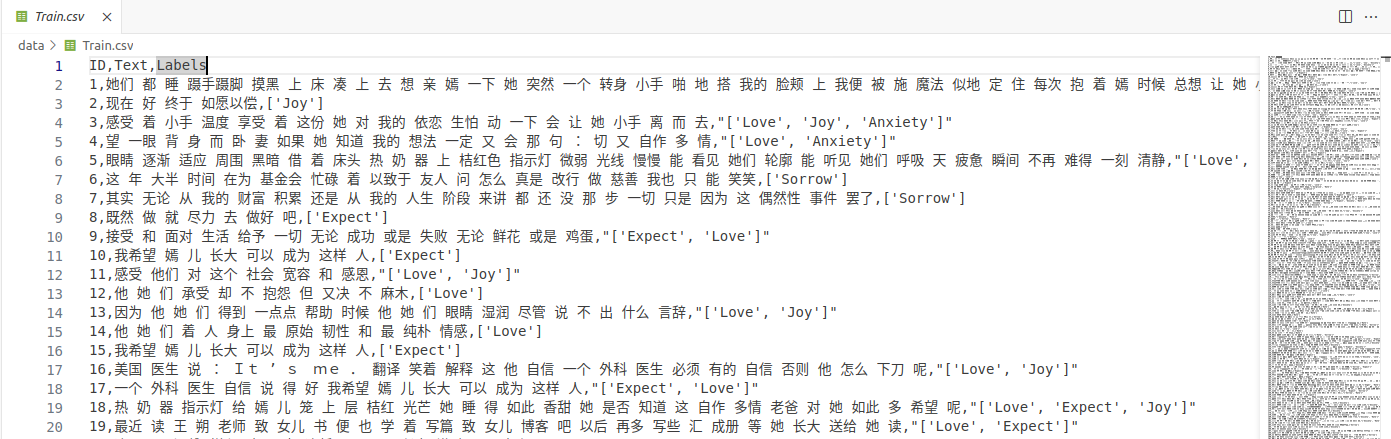
\includegraphics[width=0.8\textwidth]{logos/2024-01-01_21-35.png}
        \caption{train dataset demonstration}
        \label{fig: ERNIE 3.0 framework}
    \end{figure}

  Validate the algorithm's feasibility and assess its performance on the given dataset. 
  
  The provided test dataset consists of 26,000 entries, each presented in the form of [id, text, label]. Thirty percent of the data is randomly allocated for validation, and the remaining 70\% is designated as the training set. For each sample (a row in the CSV file), the value of the text field is processed by trimming leading and trailing whitespaces, removing spaces generated by the pre-tokenization of the dataset, and subsequently inputting it into a tokenizer to generate word vectors. The labels are one-hot encoded.
  
  Following this process, the pre-trained model is fine-tuned on the partitioned test set, and the optimal model is selected through validation. The saved optimal model is then employed for inference on the test set, comprising 6,153 entries in the format [id, text]. The model outputs the one-hot encoded form of the labels corresponding to the text field, which is then binarized into readable labels based on a given threshold.

    

  \end{block}

     \begin{block}{Code Availability}

   The data, code, and models involved in this project have been open-sourced. 
   
       The repository can be found at \href{https://github.com/hilinxinhui/kdd}{https://github.com/hilinxinhui/kdd}. 
   
   Feel free to raise any questions or provide feedback by submitting an issue on the repository.


  \end{block}

\end{column}

\separatorcolumn

\begin{column}{\colwidth}

  

  \begin{block}{Model \& Algorithm}

    \begin{figure}
        \centering
        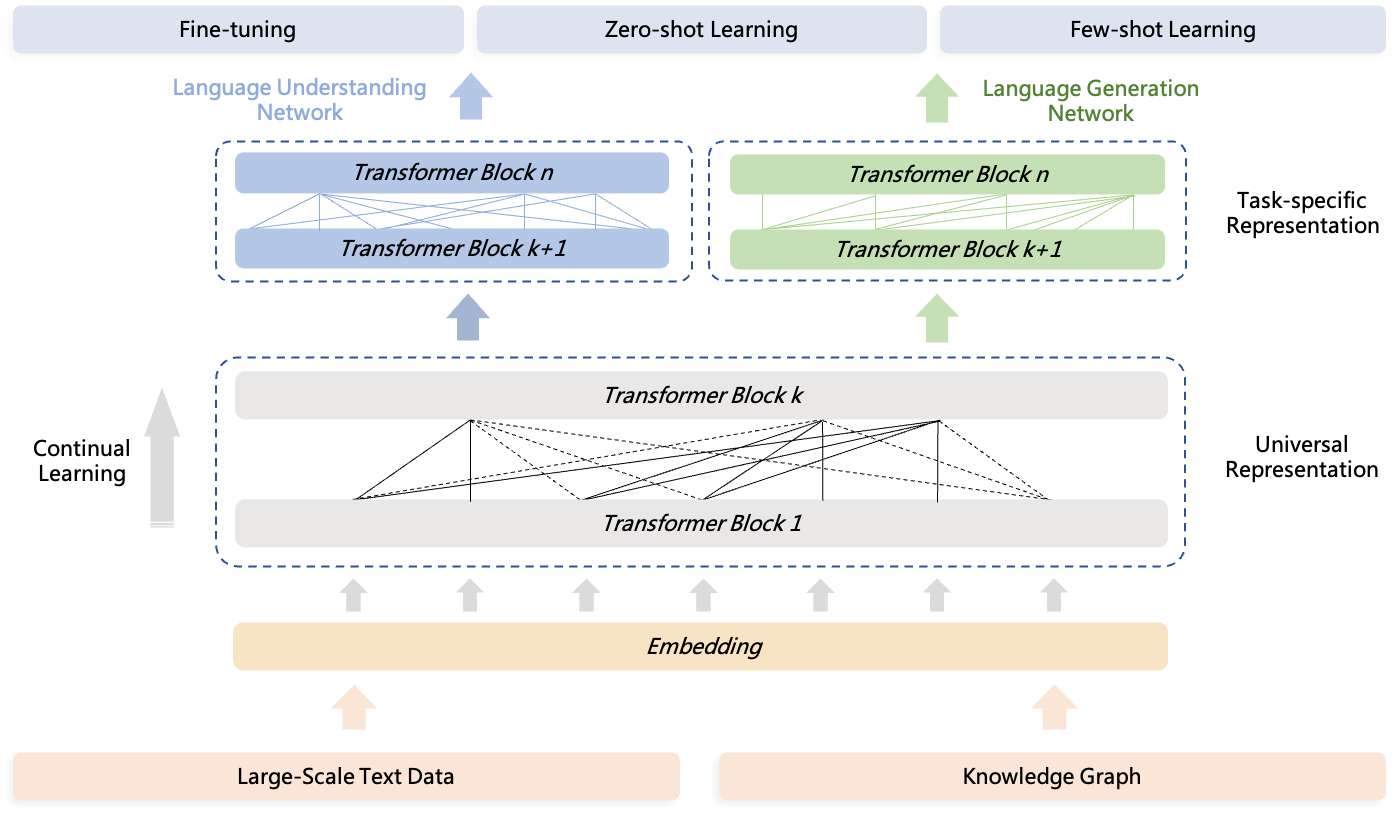
\includegraphics[width=1\textwidth]{logos/ernie-framework.png}
        \caption{ERNIE 3.0 framework}
        \label{fig: ERNIE 3.0 framework}
    \end{figure}

% Algorithm 1: Fine-tuning Stage
\begin{algorithm}[H]
  \caption{Fine-tuning Stage}
  \label{alg:fine-tuning}
  \begin{algorithmic}[1]
    \REQUIRE Pre-trained model, labeled downstream task training set
    \ENSURE Fine-tuned model
    \STATE Data cleaning: Remove invalid characters, pre-tokenization, generate word vectors for input text, and create one-hot encoding for labels.
    \STATE Split the training set into training and validation sets.
    \STATE Train the pre-trained model with input word vectors. Test the model on the validation set every 50 steps, measuring AUC, F1-Score, Precision, and Recall scores.
    \STATE Save the model with the highest F1-Score on the validation set as the fine-tuned model.
  \end{algorithmic}
\end{algorithm}

% Algorithm 2: Inference Stage
\begin{algorithm}[H]
  \caption{Inference Stage}
  \begin{algorithmic}[1]
    \REQUIRE Fine-tuned model, unlabeled downstream task test set
    \ENSURE Labels for the downstream task test set
    \STATE Preserve all hyperparameters from data processing. Perform word embedding and one-hot encoding on the test set.
    \STATE Use the fine-tuned model from Algorithm 1 to predict labels for the generated word vectors.
    \STATE Apply the sigmoid activation function to the predicted labels and binarize according to a given threshold.
    \STATE Generate original labels corresponding to the binarized results.
    \STATE Save the labels for each sample in the test set.
  
  \end{algorithmic}
\end{algorithm}

   

  \end{block}




\end{column}

\separatorcolumn

\begin{column}{\colwidth}

  \begin{block}{Experiment}

    % % Like this:

    \begin{table}
    \begin{minipage}{0.48\linewidth}
      \centering
      \begin{tabular}{l r r c}
        \toprule
        \textbf{Hyperparameter} & \textbf{Value} \\
    \midrule
    Maximum Tokenizer Sequence Length & 100 \\
    Test Set Batch Size & 16 \\
    Validation Set Batch Size & 16 \\
    Initial Learning Rate & 2e-5 \\
    Learning Rate Decay Rate/Epochs & 0.5 \\
    Optimizer & AdamW \\
    Loss Function & BCEWithLogitsLoss \\
    Fine-tuning Epochs & 4 \\
    Inference Binarization Threshold & 0.38 \\
        \bottomrule
      \end{tabular}
      \caption{table of hyperparameters}
      \end{minipage}
      \begin{minipage}{0.48\linewidth}
      \centering
      \begin{tabular}{l r r c}
        \toprule
        \textbf{Metrics} & \textbf{Score} \\
        \midrule
         AUC & 0.91337 \\
    F1-Score & 0.67598 \\
    Precision & 0.64911 \\
    Recall & 0.70517 \\
        \bottomrule
      \end{tabular}
      \caption{performance on validation set}
      \end{minipage}
    \end{table}

    % \begin{table}
    %   \centering
    %   \begin{tabular}{l r r c}
    %     \toprule
    %     \textbf{Metrics} & \textbf{Score} \\
    %     \midrule
    %      AUC & 0.91337 \\
    % F1-Score & 0.67598 \\
    % Precision & 0.64911 \\
    % Recall & 0.70517 \\
    %     \bottomrule
    %   \end{tabular}
    %   \caption{A table caption.}
    % \end{table}



  \end{block}

    \begin{block}{Future Works}

\begin{enumerate}
    \item \textbf{Optimizing Model Generalization:} Explore alternative models like TextCNN or RNNs on the limited dataset provided to achieve comparable test accuracies, addressing the challenge of model overfitting due to the mismatch between model parameters and dataset size.
    
    \item \textbf{Adapting to Downstream Tasks Efficiently:} Future research can focus on fine-tuning specific layers of the base model to enhance adaptability to specific sentiment classification tasks, avoiding the introduction of unrelated tasks during pre-training.
    
    \item \textbf{Enhancing Training and Inference Efficiency:} Efforts can be directed towards improving efficiency in both model training and inference. Consider using parallel hardware acceleration during training and implementing model quantization for performance optimization during inference.
\end{enumerate}


  \end{block}



  \begin{block}{References}
% List the references with the \textbf{BibTeX} format in the file named \textbf{poster.bib}.
    \nocite{*}
    \footnotesize{\bibliographystyle{plain}\bibliography{poster}}

  \end{block}

\end{column}

\separatorcolumn
\end{columns}
\end{frame}

\end{document}
